\chapter{Metodologia} \label{Metodologia}

Neste capítulo será apresentada a formulação geral do problema de Transferência de Coordenadas, bem como a solução proposta para detecção das manobras realizadas em uma corrida.

\section{Formulação do Problema e metodologia}

Trabalhos anteriores (citar) que se utilizaram de smartfones para realizar a coleta de informações a respeito do comportamento do motorista, não levaram muito em consideração a calibração correta dos eixos do aparelho com o carro. Muitas das vezes, Lançando-se mão de que para descrever os padrões de direção de um veiculo, o alinhamento manual do eixo do telefone, para com o do veículo pode ser suficiente. No entanto, o objetivo do presente trabalho consiste em aplicar um método consistente para se obter a detecção de manobras independente da posição do celular no carro. Nesse sentido uma troca de bases se faz necessária.

Definiu-se o cenário de aplicação de que para cada viagem, o aparelho celular pode estar posicionado em qualquer desconhecido, no entanto fixo.

\section{Transferência de Coordenadas}

A principio não se pode compreender a dinâmica veicular através da leitura de sensores, a não ser que o sistema de coordenadas do telefone esteja alinhado com o do veículo. A princípio se propõem em realizar o alinhamento dos eixos utilizando o giroscópio e o acelerômetro.

O sistema de coordenadas do telefone ($X_t,Y_t,Z_t$) é determinado pela posição do mesmo, no interior do veículo. O alinhamento do coordenadas consiste em encontrar a matriz de rotação que alinha o sistema de coordenadas do telefone com o do Veículo ($X_v,Y_v,Z_v$). 

Primeiramente, define-se um vetor unitário de três coordenadas no sistema de coordenadas do veículo, $\hat{i}$,$\hat{j}$ e $\hat{k}$.(por exemplo com $\hat{i} = [1,0,0]$ no sistema de coordenadas do veículo). Denotamos as coordenadas correspondentes desse vetor unitário no sistema de coordenadas do telefone como:

\begin{equation}
    \hat{q} = [x_q,y_q,z_q]
\end{equation}{}

onde $\hat{q} \in i,j,k$  dessa forma a matriz de rotação é dada por:

\begin{equation}
    R = \begin{Bmatrix}
x_i &x_j  &x_k \\ 
y_i &y_j  &y_k \\ 
z_i &z_j  &z_k 
\end{Bmatrix}
\end{equation}{}

Para se obter cada elemento da matriz de rotação, utilizamos medições de acelerômetro e do giroscópio.

\subsection{Derivando Aceleração Gravitacional} 
Pode ser obtido utilizando um filtro de passa-baixa(exemplo: suavização exponencial) nos três eixos do acelerômetro para se obter as componentes constantes nesses três eixos, de forma a se encontrar a gravidade, atuante sobre o smartfone. Essa medição é realizada nos primeiros instantes em que o celular se encontra parado. Então é possível obter-se a média dos três eixos que é então normalizada de forma a gerar o vetor unitário $\hat{k} = [x_k,y_k,z_k]$  

\begin{figure}
    \centering
    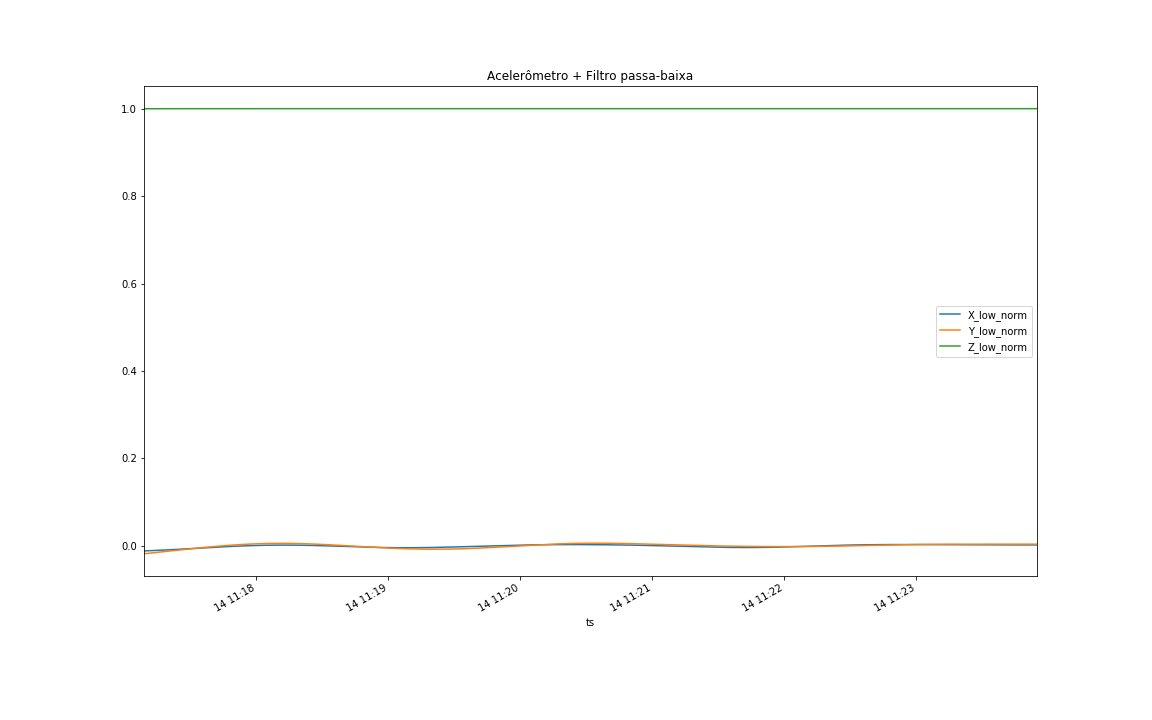
\includegraphics[width=150mm]{Figuras/acelerometroPassaBaixa.png}
    \caption{Medições dos três eixos do Acelerômetro após aplicação do filtro passa-baixa. }
    \label{fig:acelerometroPassaBaixa}
\end{figure}

\subsection{Derivando Aceleração Longitudinal}
Para se obter $\hat{j}$ lançamos mão do fato de que as leituras nessa direção de movimento do veículo são dadas quando aceleramos ou desaceleramos com o carro em linha reta. Quando o celular é colocado no painel do veículo ou montado em algum suporte, com o carro ligado, ele é submetido a um determinado nível de vibração, que varia de veículo para veículo. Quando se acelera em linha reta, os primeiros micro segundos dessa aceleração longitudinal pode ser observada em termos da magnitude da aceleração linear. que, nesse momento, é essencialmente um vetor que aponta na direção do movimento do carro, e tipicamente maior do que o ruido observado quando o carro ainda se encontra em repouso. 

Em vista da característica ruidosa do acelerômetro, Não é possível estimar o vetor velocidade - que possui o mesmo sentido do movimento do carro - com acurácia; o erro numérico da integração se acumula de forma rápida, tornando a medição imprecisa. No entanto, a direção do vetor velocidade pode ser estimada através dessa integração, e por mais que o erro numérico mascare o valor real da velocidade, sua direção continua condizente com a direção de movimento do veículo. Para o calculo da integral, podemos utilizar o giroscópio para determinar se o veículo está se locomovendo em linha reta; nesse caso a magnitude do giroscópio é muito próxima de zero, e em seguida encontramos o instante onde o veículo acelera, encontrando $\hat{j} = [x_j,y_j,z_j]$. De acordo com (citar autor) deve-se excluir a componente da gravidade que pode se distribuir em todos os três eixos do telefone, dessa forma tornando o modelo robusto ao plano inclinado.



\begin{figure}
    \centering
    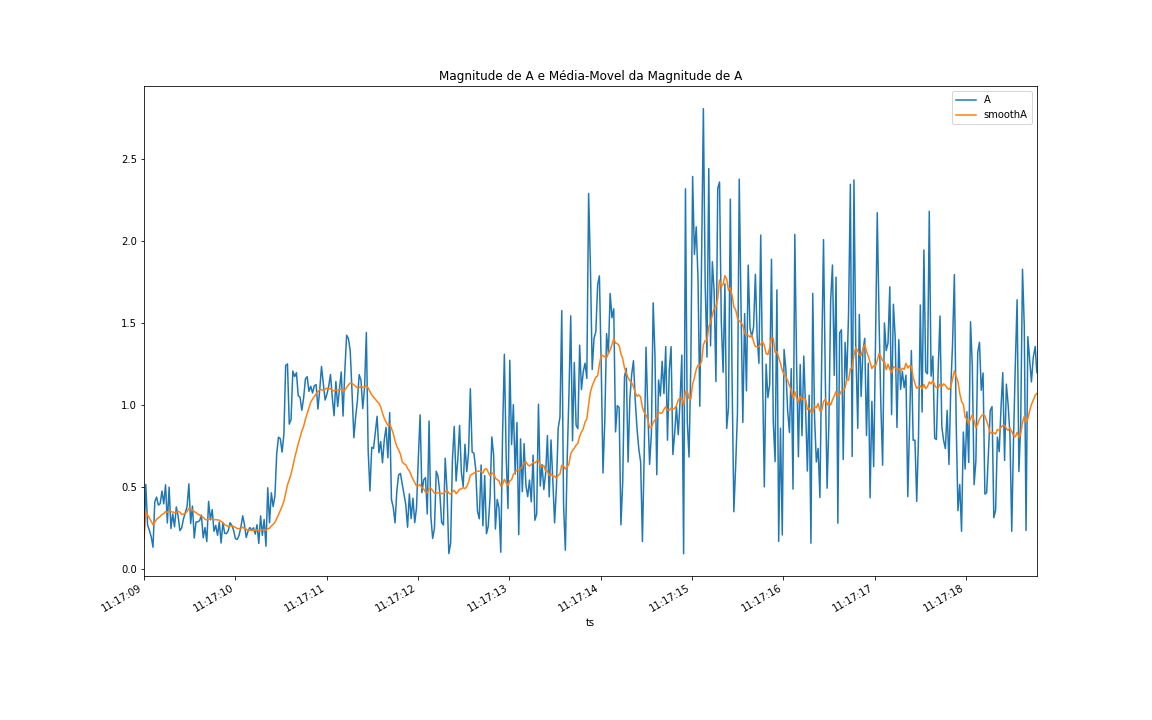
\includegraphics[width=150mm]{Figuras/acelerometroMediaMovel.png}
    \caption{Magnitude da Aceleração Linear com e sem filtro de passa-baixa}
    \label{fig:acelerometroMediaMovel}
\end{figure}

\subsection{Derivando Aceleração Lateral}
Como o sistema de coordenadas segue a regra da mão direita, $\hat{i} =\hat{j} \times \hat{k} = [x_i,y_i,z_i]$.

Depois de se obter a matriz de rotação $R$ Nós podemos obter a leitura dos sensores \begin{equation}
    s^{'} = s \times R \label{eq:trocaDeBase}
\end{equation}

 Deve-se frisar que, o escopo do presente trabalho não contempla o caso onde o dispositivo se encontra não fixo no carro (ex.: na mão do motorista). Quando é detectada algum pico na magnitude do giroscópio maior do que o limiar de 1.5 rad/s, o aparelho deve ser considerado como descalibrado e a transferência de coordenadas deve ser reestimada. Uma vez que um pico dessa magnitude pode representar que a posição do telefone foi alterada. Dado que a média magnitude do giroscópio se mantém próximo a 0 na maior parte da viagem chegando a 0.5-0.6 rad/s em momentos de curva.


\section{Teste da Transferência de Coordenadas no Conjunto de Dados Aberto}
A fim de se confirmar o método de transferência de coordenadas proposto se utilizou, a princípio, os dados coletados em trabalhos anteriores \cite{junior2017driver}. O conjunto de dados coletados em questão consiste em 4 viagens experimentais de aproximadamente 13 minutos cada, onde se executaram diversas manobras agressivas de direção. Para tal experimento foi-se utilizado o veículo Honda Civic 2011. Para captura de dados utilizou-se um aparelho Motorola XT1058 com Android versão 5.1. O aparelho em questão foi fixado no para-brisa do veículo durante a viagem, por meio de um suporte, e o mesmo não foi movido ou operado durante a captura dos sensores. A taxa de amostragem dos sensores variou entre 50 a 200 Hz, a depender do sensor. Os carros foram dirigidos por dois motoristas com 15 anos de experiência. O dia em que o experimento ocorreu era ensolarado. Ressaltando-se que os dados coletados de acelerômetro e giroscópio neste experimento estavam no sistema de coordenadas Global; ou seja, o eixo Z apontando para o centro da terra, Y para o norte magnético e X sendo ortogonal aos dois primeiros.

Para se obter as medições da aceleração linear e da gravidade atuante sob o smartfone, utilizou-se respectivamente um filtro passa-alta e um filtro passa-baixa. Permitindo-se assim a obtenção dos sensores "virtuais".

Com isso, buscou-se identificar os momentos em que a magnitude da velocidade angular, medida pelo giroscópio, era baixa; ou seja, o aparelho se encontrava essencialmente parado, e um pico da magnitude da aceleração linear - nesse caso, suavizada com uma média móvel - que estivesse 2 vezes acima do patamar registrado antes de iniciar o movimento do carro \ref{fig:janelaCalibracao}.

\begin{figure}
    \centering
    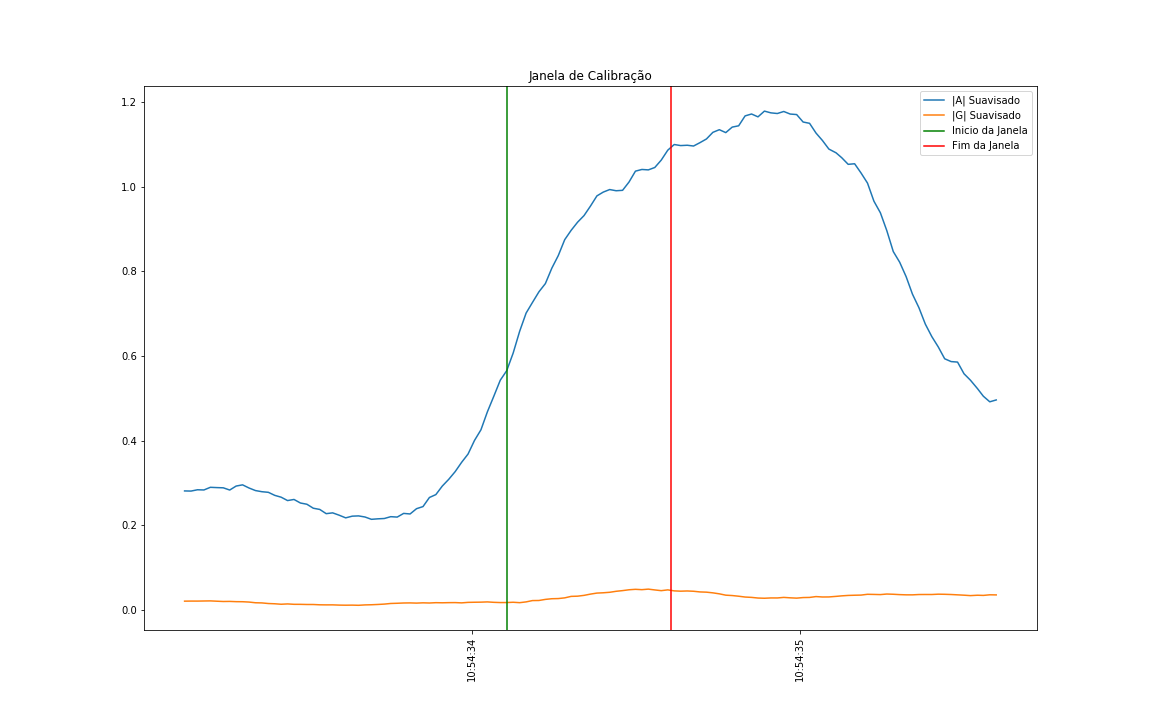
\includegraphics[width=150mm]{Figuras/janelaCalibracao.png}
    \caption{Janela em que os dados para gerar a matriz de rotação são capturados.}
    \label{fig:janelaCalibracao}
\end{figure}

Desse momento se inicia uma janela de 500ms. Ao fim da janela são estimados $\hat{i}$,$\hat{j}$,$\hat{k}$, por fim gerando a matriz de rotação. Em seguida as medições de acelerômetro linear e giroscópio, são transformadas utilizando-se a matriz, de acordo com a equação \eqref{eq:trocaDeBase}.

\begin{figure}[H]
    \centering
    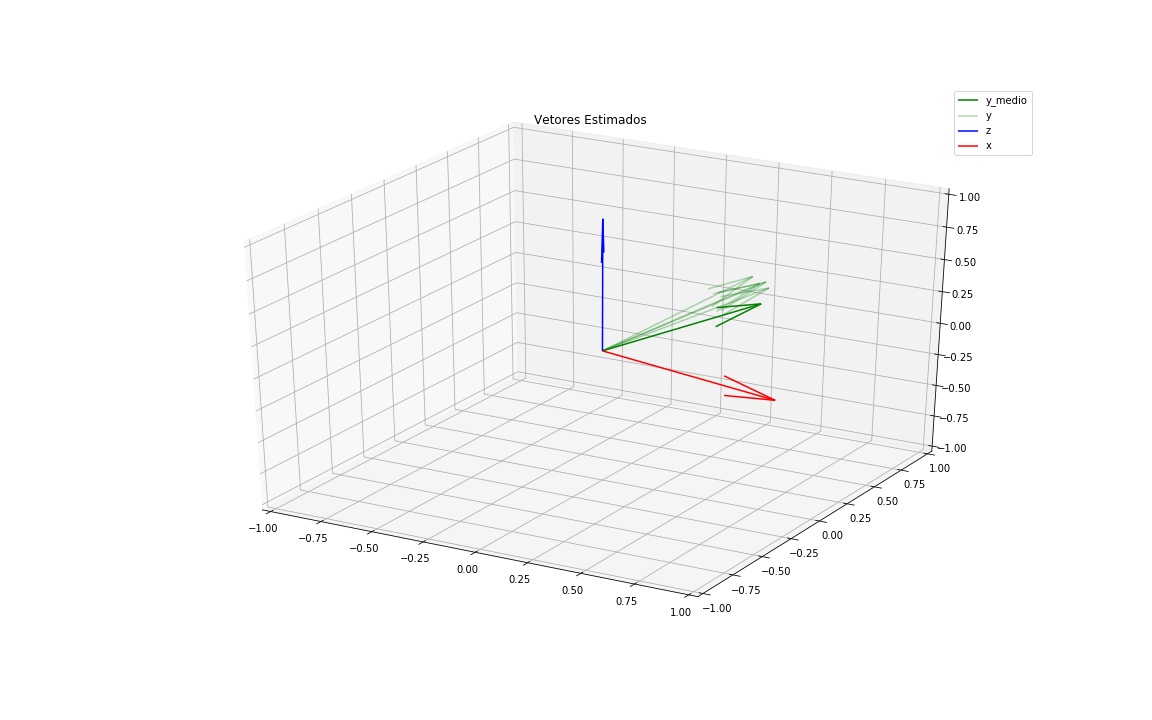
\includegraphics[width=150mm]{Figuras/vetoresEstimados.png}
    \caption{Vetores estimados para matriz de rotação.}
    \label{fig:vetoresEstimados}
\end{figure}{}

\begin{figure}[H]
    \centering
    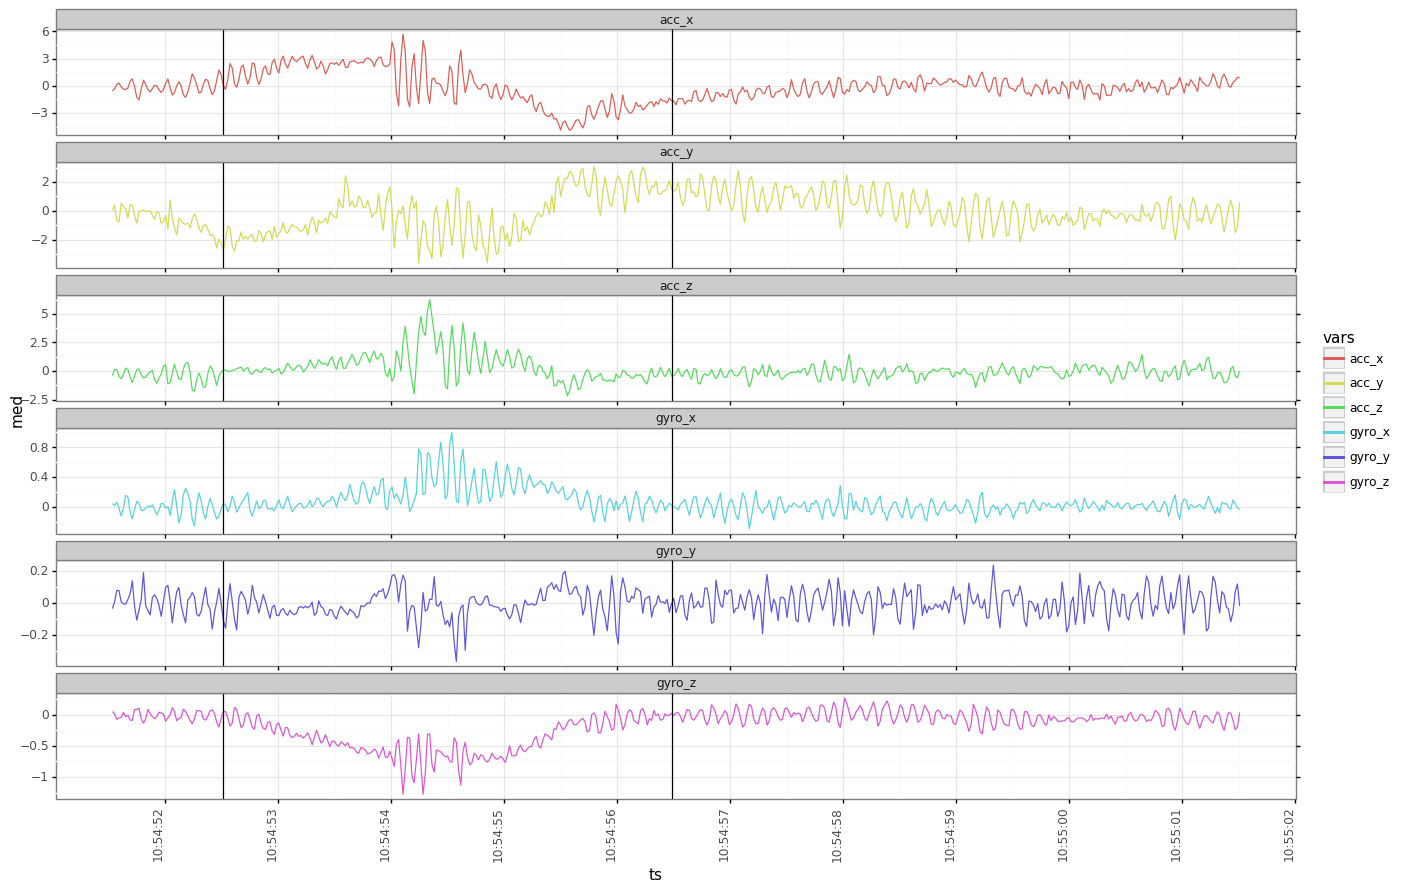
\includegraphics[height=110mm]{Figuras/assinaturaCurvaDireita.png}
    \caption{Assinatura de Curva Direita com os dados de sensor rotacionados.}
    \label{fig:assinaturaCurvaDireita}
\end{figure}{}

\section{Teste da Transferência de Coordenadas no Conjunto de Dados Próprio}

Para um segundo experimento, dessa vez com dados próprios, se utilizou o aplicativo "Sensor Record" que permite a gravação de diversos sensores do dispositivo Android. No caso, utilizou-se um aparelho Xiaomi Mi 8 Lite, gravando os dados do sensor de giroscópio, acelerômetro linear e gravidade, presentes no dispositivo, a uma frequência de amostragem média de 100 Hz. O veiculo utilizado no experimento foi um Toyota Corolla 2005. Todas as viagens foram realizadas pelo mesmo motorista, com mais de 20 anos de experiência. Os dados foram gravados na parte do dia em uma corrida que compreendia um percurso de aproximadamente 1km. O smartfone foi disposto em 3 posições em termos do seu sistema de coordenadas como descrito a seguir e observado na Figura \ref{fig:posicoesCelular};

\begin{itemize}
    \item Alinhado com o veículo
    \item Deitado sob o painel com sua coordenadas X alinhada com a coordenada Y do carro
    \item Posição genérica
\end{itemize}{}

Nos três casos foi-se utilizado o método desenvolvido para se estimar a matriz de rotação. Que consiste em identificar o instante em que o veículo se encontra essencialmente parado, e monitorar a magnitude da aceleração sentida pelo aparelho. No momento em que essa magnitude for 2 vezes maior que a vibração normal do carro - registrada a partir dos primeiros instantes que o celular se encontra parado. Assim sendo, é possível integrar a aceleração por um período curto de tempo, com o objetivo de se estimar a direção do carro. Nesse momento também se toma a média do vetor gravidade atuante sobre o dispositivo. Por fim é possível se estimar uma matriz de rotação que transforma as coordenadas do celular para as coordenadas do carro.

\begin{figure}[h]
    \centering
    \subfloat[Posição 1 (Alinhado).]{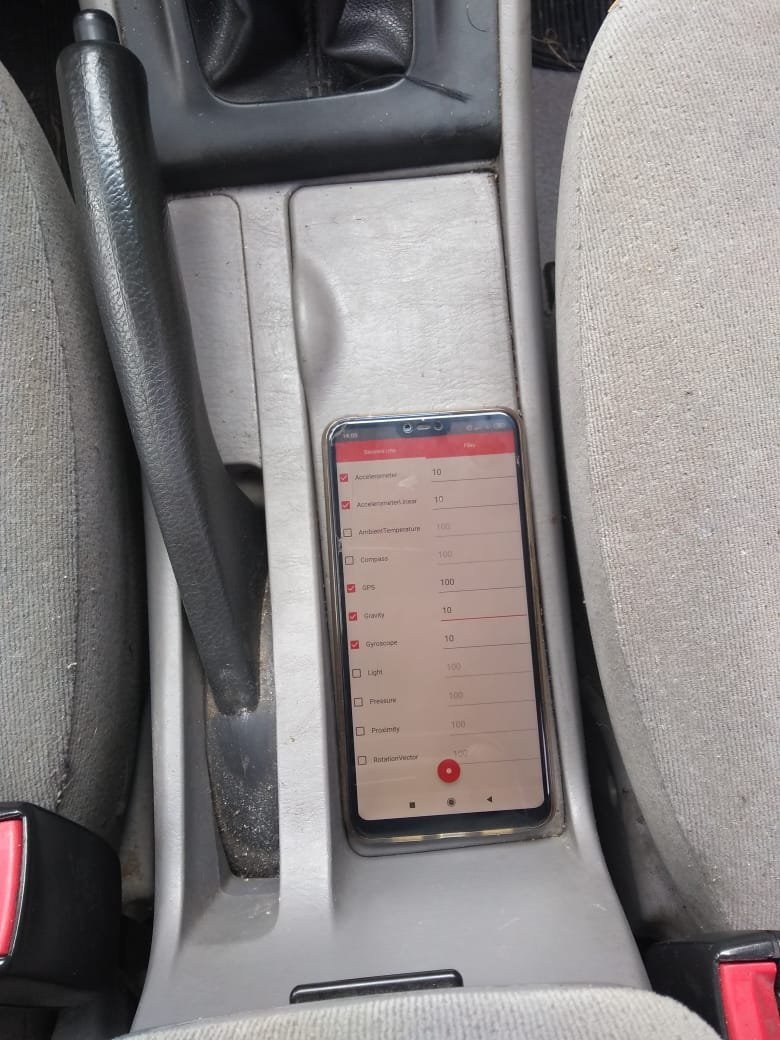
\includegraphics[width=0.3\textwidth]{Figuras/cellPosition1.jpeg}}
    \hfill
    \subfloat[Posição 2 (Deitado).]{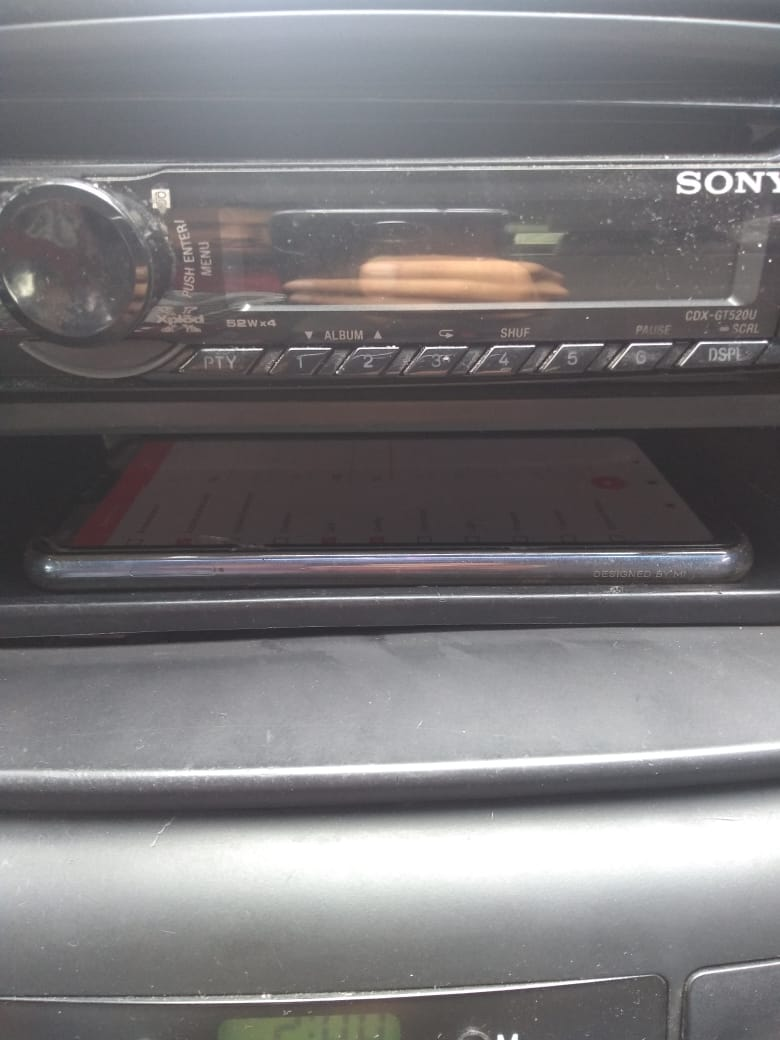
\includegraphics[width=0.3\textwidth]{Figuras/cellPosition2.jpeg}}
    \hfill
    \subfloat[Posição 3 (Genêrica).]{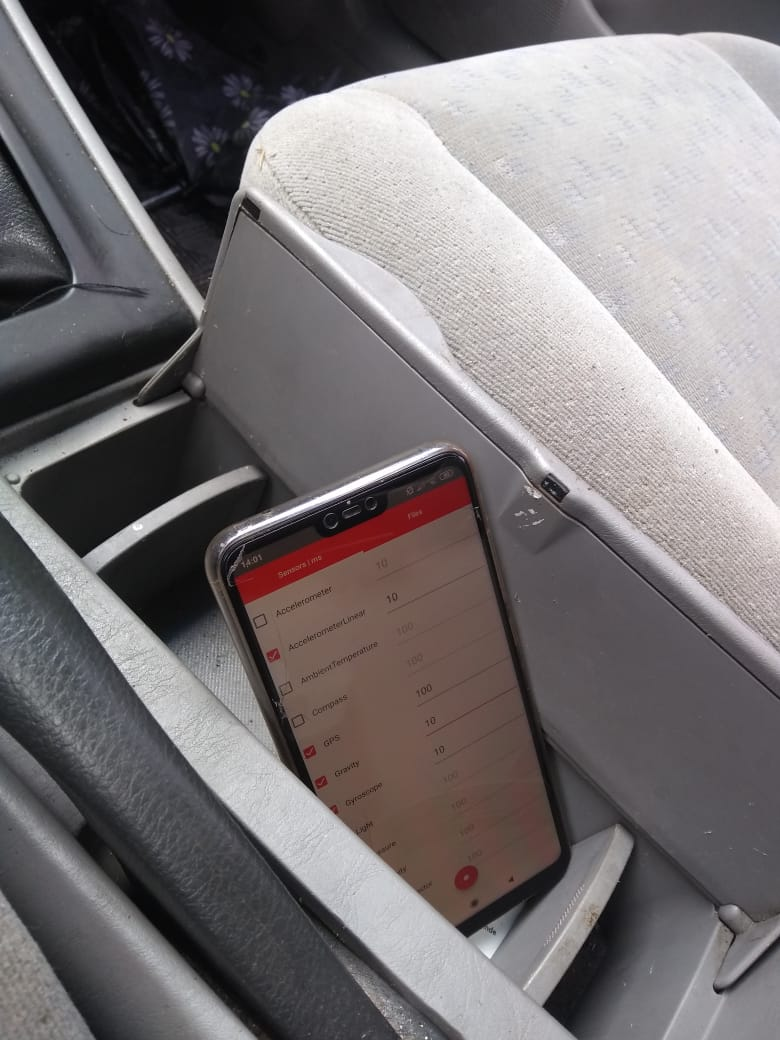
\includegraphics[width=0.3\textwidth]{Figuras/cellPosition3.jpeg}}
    \caption{Posições do Celular}
    \label{fig:posicoesCelular}
\end{figure}{}

De forma a se obter validação do método para troca de coordenadas, se observou: O coeficiente de correlação de Pearson dos dados rotacionados - no caso dos eixos conhecidos; a quantidade de energia em Y - uma vez que as corridas se deram no mesmo percurso e em condições muito parecidas, elas tendem a ser próximas; a direção das curvas, uma vez que o percurso consiste em uma volta em um quarteirão, haverão 4 assinaturas de curva para direita, tanto pelo eixo Z rotacionado do giroscópio, quanto pelo eixo X rotacionado do acelerômetro; dessa forma permitindo identificar se a troca de base foi ou não bem sucedida.


